\section{Competition creates research}\label{sec:research}

So far the investor is present with a fixed probability \(\lambda\); now the investor chooses that probability and
pays for it. Before it learns the class, the investor chooses a research intensity \(\lambda\in[0,\lb]\) at the
cost \((a/2)\lambda^2\), where \(a>0\) and the cap satisfies \(0<\lb<1\). Research succeeds with probability
\(\lambda\), independently of the class, the costs and the incumbent's value. A success reveals the class, and the
investor then fills the slot with an order. After a failure, a liquidity trader fills the slot.

Research is therefore the presence probability of Section~\ref{sec:slot}, chosen at a cost. It is the specialist's
own work on the target's customers, technology and demand, and it must end before the order opportunity. The cap
\(\lb\) is the probability that this work can reveal the class at all before the challenger decides, because some
facts about the match become visible only through the buyer's own diligence. The marginal cost rises because the
specialist uses cheap sources first, such as its sector coverage, and costly ones later, such as expert calls. The
quadratic cost is the simplest form whose marginal cost rises.

A success takes the place of a liquidity order because the opportunity has room for one order. An investor that
knows the class takes it. After a failure, the investor knows no more than the market, so an order would lose at
least its cost \(k\). The opportunity then passes to a liquidity trader. More research therefore also removes
liquidity orders, and it reduces the camouflage of the investor's own orders.

Market makers and the challenger do not observe the research choice, so they price and decide at a conjectured
intensity; throughout this section the prior is \(1/2\). In an equilibrium with research, the conjectured
intensity is the investor's best research choice at the equilibrium prices and entry rule, and the order after
a success is optimal, including after a deviation from zero research.
The best research choice is unique: it equals the expected trading payoff after a success divided by \(a\), capped
at \(\lb\), so research never has a tie. Appendix~\ref{app:research} states the equilibrium with research
formally and gives each result of this section in full.

Research raises the top posterior that a purchase can reach. At intensity \(\lambda\), I write \(M_\lambda\) for
that top posterior and \(m_\lambda=1-M_\lambda\) for the bottom posterior, the posterior bounds of
Section~\ref{sec:inference} at the prior \(1/2\) when the presence probability is \(\lambda\). When
\(1/2<\tau(r)<1\), the \emph{recruitment intensity} \(\lambda_E(r)\) is the research level at which a full purchase
just reaches the threshold, \(M_\lambda=\tau(r)\), so a full purchase recruits exactly when research is at least
\(\lambda_E(r)\).

Suppose that class \(H\) buys after a success, class \(L\) abstains, and only a purchase recruits. A purchase
then earns \(\DT(r)m_\lambda-k\), and research optimality at an interior intensity reads:
\begin{equation}\label{eq:research}
2a\lambda=\DT(r)\,m_\lambda-k .
\end{equation}
The left side rises with \(\lambda\), and the right side falls, because more research removes camouflage. When
\(\DT(r)>2k\), the two sides meet at one intensity \(\lambda_R(r)\in(0,1)\).

On the branch where only a purchase recruits, a wider target-payoff spread raises the return to a purchase, so
the investor chooses more research and a purchase becomes more likely; research, entry and high-class ownership
then rise together with incumbent strength. At the benchmark strengths, the same force takes the economy from no
research and no trade against the weak incumbent, through coexistence of zero research with the research branch at
intermediate strengths, to research at the cap with trade in both directions against the strong and the very
strong incumbent. The benchmark research parameters are \(a=\reg{res_a}\) and the cap \(\lb=\reg{res_cap}\), the
presence probability of Section~\ref{sec:benchmark}, so research at the cap reproduces the benchmark slot.

\begin{proposition}[Competition creates research]\label{prop:research}
Let the auction be the benchmark auction at the prior \(1/2\), and suppose that \(0<\beta\le1/3\) and \(a>0\).
\begin{enumerate}[label=(\alph*),leftmargin=2em]
\item On the strengths with \(\DT(r)>2k\), research \(\lambda_R(r)\) is continuously differentiable and rises
strictly in \(r\). Wherever the research branch is an equilibrium, entry
\(\rho+(1-\rho)\bigl[\beta+(1/2-\beta)\lambda_R(r)\bigr]\) and high-class ownership
\(\tfrac12[\rho+(1-\rho)(\beta+(1-\beta)\lambda_R(r))]\) rise strictly with \(r\).
\item At the benchmark, with the research cost \(a=\reg{res_a}\) and the cap \(\lb=\reg{res_cap}\):
\begin{enumerate}[label=(\roman*),leftmargin=2em]
\item At \(r_0\), the unique equilibrium has no research and no trade. Entry is \(\rho\).
\item At each \(r\in\{\reg{str_r155},\reg{str_r160},\reg{str_r165}\}\), there are exactly two equilibria. In the
first, the investor does no research, and entry is \(\rho\). In the second, the research branch, research is
\(\lambda_R(r)\), with \(\lambda_E(r)<\lambda_R(r)<\lb\). After a success, class \(H\) buys and class \(L\) abstains,
only a purchase recruits, and entry is \(\rho+(1-\rho)[\beta+(1/2-\beta)\lambda_R(r)]\).
\item At \(r_1\) and \(r_2\), the unique equilibrium has research at the cap and trade in both directions. It is the
equilibrium of Proposition~\ref{prop:ccc} with \(\lambda=\lb\). Entry is \(\reg{res_entry_r1}\) at \(r_1\) and
\(\rho\) at \(r_2\).
\end{enumerate}
\end{enumerate}
\end{proposition}

At \(r_0\) every nonzero order after a success loses, so the expected trading payoff after a success is zero and
the best research choice is zero. At the intermediate strengths, the equilibrium without research confirms itself: against an
uninformative price the best nonzero order after a success earns \(\rho\DT/2-k<0\), because these strengths lie
below \(r_N\); on the research branch, a purchase reveals enough to recruit, and its return pays for the research
that makes it informative.

At \(r_1\) and \(r_2\), a bound on every candidate profile makes a full order profitable net of the marginal
research cost at the cap. Every trade
choice at the six strengths is strict, so the lists do not depend on how an indifferent investor breaks a tie.

\begin{table}[tbp]
\centering\small\singlespacing
\caption{Research and entry at the intermediate strengths.}\label{tab:research}
\begin{tabular}{@{}lccc@{}}
\toprule
 & \(r=\reg{str_r155}\) & \(r=\reg{str_r160}\) & \(r=\reg{str_r165}\)\\
\midrule
Target-payoff spread \(\DT(r)\) & \reg{res_Delta_r155} & \reg{res_Delta_r160} & \reg{res_Delta_r165}\\
Preparation threshold \(\tau(r)\) & \reg{res_tau_r155} & \reg{res_tau_r160} & \reg{res_tau_r165}\\
Recruitment intensity \(\lambda_E(r)\) & \reg{res_lamE_r155} & \reg{res_lamE_r160} & \reg{res_lamE_r165}\\
Research \(\lambda_R(r)\) & \reg{res_lambda_r155} & \reg{res_lambda_r160} & \reg{res_lambda_r165}\\
Posterior after a purchase \(M_{\lambda_R}\) & \reg{res_muplus_r155} & \reg{res_muplus_r160} & \reg{res_muplus_r165}\\
Entry on the research branch & \reg{res_entry_r155} & \reg{res_entry_r160} & \reg{res_entry_r165}\\
High-class ownership on the branch & \reg{res_own_r155} & \reg{res_own_r160} & \reg{res_own_r165}\\
Entry without research & \reg{entry_r0} & \reg{entry_r0} & \reg{entry_r0}\\
\bottomrule
\end{tabular}
\par\medskip
\begin{minipage}{0.92\linewidth}\footnotesize
\textit{Notes.} The benchmark with \(a=\reg{res_a}\) and \(\lb=\reg{res_cap}\). The spread, the threshold and
\(\lambda_E\) are exact rationals; research and the values that depend on it are interval enclosures rounded to six
places.
\end{minipage}
\end{table}

Research and entry rise together across the three intermediate strengths in Table~\ref{tab:research}: research
rises from \(\reg{res_lambda_r155}\) through \(\reg{res_lambda_r160}\) to \(\reg{res_lambda_r165}\), and entry rises
from \(\reg{res_entry_r155}\) through \(\reg{res_entry_r160}\) to \(\reg{res_entry_r165}\). A stronger incumbent
widens the target-payoff spread, so a purchase earns more and the investor chooses more research; the posterior
after a purchase then rises above the threshold by more, and a purchase becomes more likely. Part (a) of
Proposition~\ref{prop:research} shows that this comovement is general along the branch.

The slope of entry is \((1-\rho)(1/2-\beta)\lambda_R'(r)\), which is positive for every \(\beta\le1/3\). A purchase
has probability \(\beta+(1/2-\beta)\lambda\): research adds informed purchases in class \(H\) and removes liquidity
orders in both classes, and the first effect dominates.

At the benchmark, the research branch is an equilibrium exactly on \([r_R,\bar r_R)\), with
\(r_R\approx\reg{res_rR}\) and \(\bar r_R\approx\reg{res_rcap}\). The start \(r_R\) is the strength at which the purchase
posterior just reaches the threshold and the purchase also pays the marginal research cost:
\(\DT(1-\tau)=k+2a\lambda_E(r)\). The end \(\bar r_R\) is the strength at which research reaches the cap \(\lb\). Along
the branch, research rises from \(\lambda_E(r_R)=\reg{res_lambda_rR}\) to the cap, and entry rises from
\(\reg{res_entry_rR}\) to \(\reg{res_entry_cap}\). Zero research is an equilibrium along the whole branch, because
\(\bar r_R<r_N=\reg{res_rN}\). On \([\bar r_R,r_N)\), research at the cap coexists with zero research, and entry equals
\(\reg{res_entry_cap}\).

Against strong incumbents, research sits at the cap. Above a strength \(r_U\approx\reg{res_rUR}\),
a bound on every candidate profile forces full orders and research at the cap
(Appendix~\ref{app:research}).

\begin{figure}[tbp]
\centering
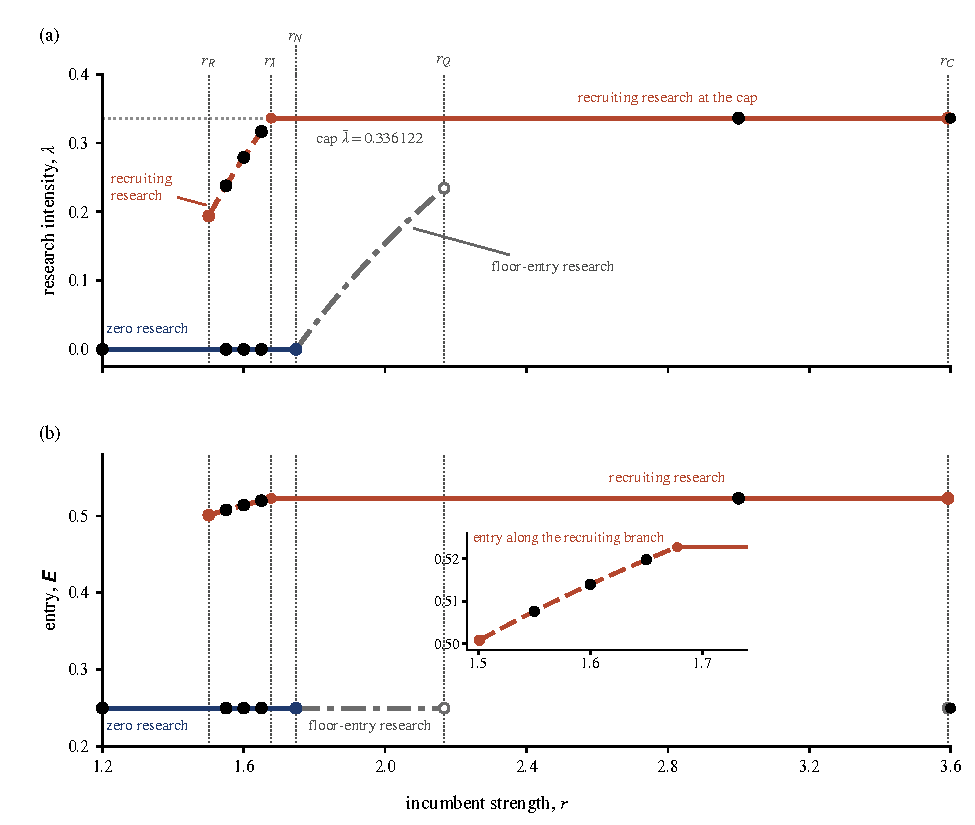
\includegraphics[width=\linewidth]{figures/research.pdf}
\caption{Research and entry along the research branch.}\label{fig:research}
\par\medskip
\begin{minipage}{\linewidth}\footnotesize\singlespacing
\textit{Notes.} The benchmark with \(a=\reg{res_a}\) and \(\lb=\reg{res_cap}\), where an indifferent high-cost
challenger prepares. Panel (a) shows research \(\lambda\), and panel (b) shows entry; the inset enlarges entry
along the research branch. Zero research is an equilibrium from \(r_0\) to \(r_N\). The research branch runs from
\(r_R\) to \(\bar r_R\). Research stays at the cap from \(\bar r_R\) to \(r_N\) and above \(r_U\); at the cap, entry
is \(\reg{res_entry_cap}\) up to the entry ceiling \(r_C\) and \(\rho\) above. Black dots mark the six strengths of
Proposition~\ref{prop:research}(b). The gray band marks the interval \((r_N,r_U)\) between the two cap ranges,
and the horizontal axis is broken there.
\end{minipage}
\end{figure}

The research branch in Figure~\ref{fig:research} starts later than the informative branch of
Section~\ref{sec:coexistence}, which starts at \(r_A=\reg{res_rA}\), because a purchase must now pay for research
as well as for trade. The two branches also adjust in different ways: with a fixed presence probability the
purchase rate adjusts through a mixture of the high class, while with research the intensity adjusts and the high
class buys with probability one after a success.

Proposition~\ref{prop:researchregion} in Appendix~\ref{app:research} gives the admissible
region of the research parameters exactly at \(\beta=\reg{beta_B}\). The equilibrium patterns of
Proposition~\ref{prop:research}(b) hold with strict margins exactly when the cap lies in the strip
\((\lambda_E(r_1),\lambda_E(r_2))\approx(\reg{res_cap_lo},\reg{res_cap_hi})\) and the cost lies in a window that
depends on the cap. At the benchmark cap, this window is \((\reg{res_a_lo},\reg{res_a_up})\). With \(1+u=\eu\), the
cap \(\lb=u\beta/(1+u\beta)\) and \(a=\reg{res_a}\), these patterns hold for every
\(\beta\in(\reg{res_beta_lo},1/3]\). Entry at \(r_1\) is \(\rho+(1-\rho)[\beta+(1/2-\beta)\lb]\).
